\documentclass{article}
\usepackage{amsmath}
\usepackage{amssymb}
\usepackage[pdftex]{graphicx}
\usepackage[]{mcode}

\pdfpagewidth 8.5in
\pdfpageheight 11in
\topmargin -1in
\headheight 0in
\headsep 0in
\textheight 8.5in
\textwidth 6.5in
\oddsidemargin 0in
\evensidemargin 0in
\headheight 50pt
\headsep 0in
\footskip .75in

\title{STA 601 - Homework 3}
\author{Kedar Prabhudesai}
\date{September 11, 2013}

\begin{document}
\maketitle

\noindent {\Large\underline{\textbf{Gamma-Poisson Model:}}}\\

\indent Data Given: $n = 44, \sum{y} = 66.$\\

\indent Prior: $\theta \sim Gamma(a,b).$ $a = 2, b = 1.$\\

\indent Posterior: $\theta|y \sim Gamma(a+\sum{y},b+n)$\\

\noindent First we plot the Posterior Density function. (All the required information is provided in the title.) \\

\begin{center}
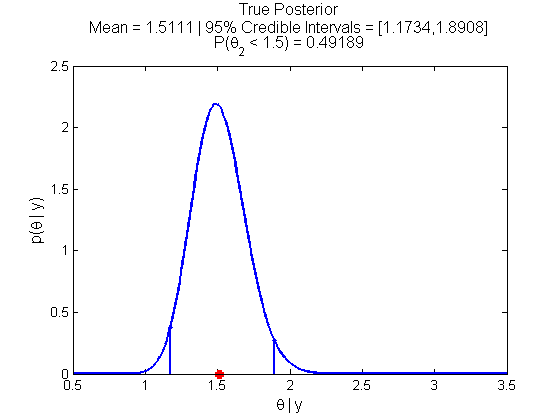
\includegraphics[scale=0.75]{Posterior.png}
\end{center}

\pagebreak

\noindent Next we will use different number of samples for MC Simulations and see the results for the same.\\

\noindent {\underline{\textbf{10 Monte-Carlo Trials:}}}\\
\begin{center}
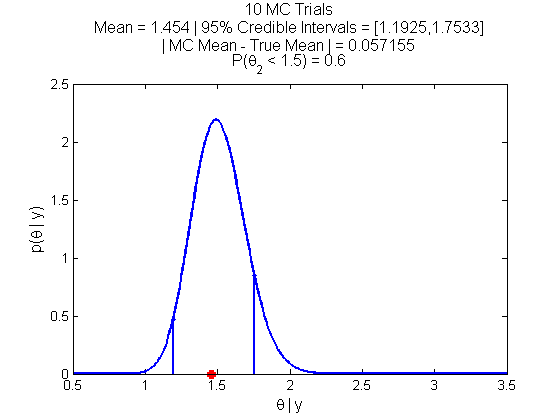
\includegraphics[scale=0.75]{MCTrials_10.png}
\end{center}

\noindent {\underline{\textbf{100 Monte-Carlo Trials:}}}\\
\begin{center}
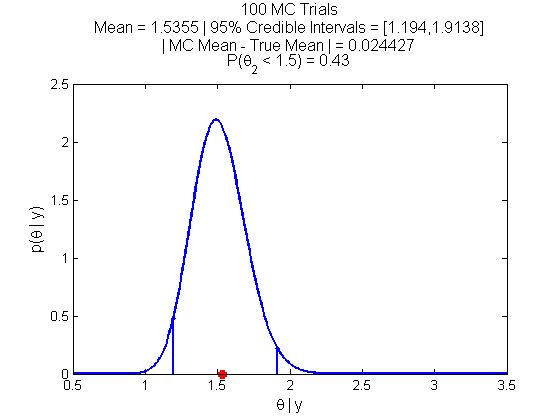
\includegraphics[scale=0.75]{MCTrials_100.png}
\end{center}

\pagebreak

\noindent {\underline{\textbf{1000 Monte-Carlo Trials:}}}\\
\begin{center}
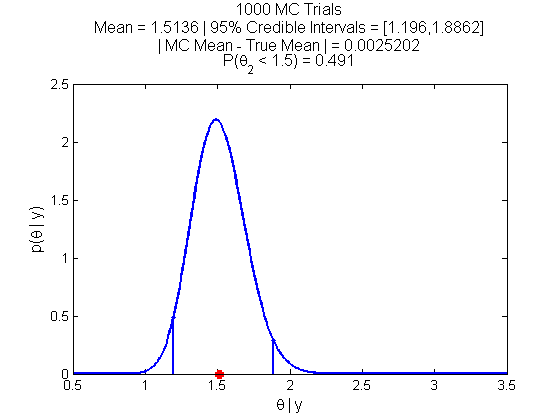
\includegraphics[scale=0.75]{MCTrials_1000.png}
\end{center}

\noindent We observe that as the number of samples increase, the absolute error between the estimated mean and the mean from MC Simulations goes down.\\

\noindent The Hoff Book provides a method to estimate the number of MC Samples to use by calculating the Monte-Carlo Standard Error. For $S = 1000$, our observed $Var[\theta|y_1,...,y_n] = 0.03226.$ 
For the difference between $E[\theta|y_1,...,y_n]$ and its MC-Estimate to be $\le0.001$ (with very high probability), the following equation should hold. $2\sqrt{0.03226/S} \le 0.001.$ Using this equation we get, $S \ge 129,078 !!!$\\

\pagebreak
\noindent {\Large\underline{\textbf{Appendix:}}}\\
\lstinputlisting{C:/Users/ksp6/Documents/Classes/2013-Fall/STA601-BayesAndModStats/homeworks/scipts/hw3.m}

\end{document}